\chapter{Diseño \label{sec:disenho}}

\section{Introducción}
Tras el análisis del panorama y las tecnologías \textit{big data} y, en especial, de las que van a ser utilizadas en este proyecto, en este apartado, se procederá con la explicación del diseño de la arquitectura \textit{big data} que, posteriormente, se implementará presentando diferentes configuraciones y alternativas.

En cuanto a la estructura de este apartado, en primer lugar procederemos a presentar una visión general del sistema y se establecerán las unidades o bloques de funcionamiento. Posteriormente, se tratará la arquitectura del sistema, teniendo en cuenta los diferentes entornos en los que seá implementado y, finalmente, se detallarán los componentes que conformarán las diferentes unidades funcionales del sistema y la interacción entre ellos para el funcionamiento del sistema.

\section{Visión general y unidades funcionales \label{unitFunc}}
Como se ha comentado en la introducción, el objetivo del proyecto es diseñar implementar una arquitectura \textit{big data} para procesar las trazas de los recorridos de taxis de la ciudad de Nueva York. Debido a la naturaleza del mismo, dónde se busca analizar diferentes configuraciones y detectar sus limitaciones, la implementación de este sistema se llevará a cabo en dos entornos diferenciados primero uno doméstico y, posteriormente, uno más realista, en la universidad.

\clearpage
Esta implementación en dos entornos hará que el diseño varíe ligeramente para cada uno de ellos, adaptándose a las condiciones técnicas que presentan. Estas diferencias solo afectarán al almacenamiento de datos por lo que la base principal de la arquitectura será la misma.

Con respecto al diseño del sistema y, también debido por el carácter experimental del proyecto se ha establecido un único rol de usuario en el sistema qué será el de administrador. Esta decisión ha sido tomada ya que no se pretende implementar el sistema para su uso en producción y, por tanto, no se ve necesaria una distinción entre tipos de usuario. Es decir, el sistema solo va a ser utilizado por un único usuario que hará todas las pruebas de rendimiento y por ello no se plantea establecer limitaciones en las funciones del sistema para otros posibles usos ni introducir nuevos roles.

En este sistema, por tanto, el administrador tendrá la capacidad de realizar los procesos de carga de datos, procesamiento de los mismos y ejecución de las consultas y obtención de resultados. Está funciones comentadas son las que darán lugar a las tres unidades funcionales del sistema (figura \ref{fig:esquemagen}), que serán las siguientes y tendrán la función descrita:

\begin{figure}[htp!]
\centering
\caption{Esquema general del sistema incluyendo las unidades funcionales}
\label{fig:esquemagen}
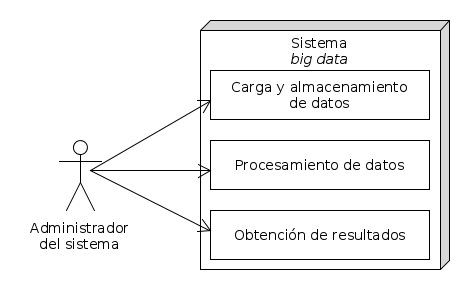
\includegraphics[scale=0.7]{diagramas/esquemaGen}
\end{figure}

\begin{itemize}
\item \textbf{Carga y almacenamiento de datos:} La carga de los datos es la primera tarea que ejecutará el usuario para que el sistema cuente con las trazas a procesar y que estas puedan ser distribuidas por los nodos. En este proyecto estos datos se corresponden con los viajes de los taxis realizados en la ciudad de Nueva York durante el año 2013 y son aportados por la organización del concurso.

En general, en los sistemas \textit{big data} el conjunto de datos proviene de diferentes fuentes, haciendo que estos tengan que ser procesados para lograr una estructura homogénea de los mismos. Sin embargo, en esta ocasión no se da el caso, donde solo se tiene un fichero \gls{CSV} con todas las trazas del año y que tienen la misma estructura.

Esta unidad, también será la encargada de almacenar los ficheros de datos cargados inicialmente por el usuario, así como, aquellos que genere el sistema. Es decir, también almacenará los ficheros procesados por el sistema y los resultados de las consultas ejecutadas.

\item \textbf{Procesado de datos:} Los datos originales tienen que ser procesados para ajustarse a los requisitos del desafío siendo, para ello, transformados y limpiados. Es decir, esta unidad, por un lado, transformará ciertos atributos de las trazas para crear nuevos a partir de los primeros, para facilitar cálculos y cumplir las normas del concurso. Por otro lado, realizará una limpieza de trazas inválidas, donde falte información o este corrupta y, también, de atributos innecesarios para los cálculos que se realizarán y, de esta forma, ahorrar espacio.

\item \textbf{Ejecución de las consultas y obtención de resultados:} Este bloque funcional es el encargado de obtener los resultados a partir del análisis de los datos contenidos en el sistema. Debido a la existencia de dos consultas, el usuario ejecutará en el sistema la consulta o consultas deseadas y este devolverá los datos de esta o estas en forma de archivo de texto plano con el nombre establecido por el usuario, que será situado en la carpeta de resultados del sistema.
\end{itemize}

\section{Arquitectura del sistema}
Gracias a las posibilidades que ofrece \textit{Apache Spark}, se ha diseñado la arquitectura ofreciendo dos posibles modos de ejecución con el fin de crear un sistema que se pueda adaptar a las diferentes situaciones que se puedan dar en cuanto a escalabilidad y disponibilidad. Esto nos permitirá además, ver las diferencias de rendimiento entre las diferentes configuraciones de forma más clara para las distintas situaciones y pruebas.

\begin{figure}[htp!]
\centering
\caption{Modos de ejecución del sistema \textit{bigdata}}
\label{fig:modoEjecución}
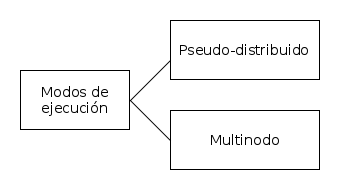
\includegraphics[scale=0.6]{diagramas/modoExec}
\end{figure}

Los dos modos de ejecución disponibles serán el pseudo-distribuido, donde solo se cuenta con un dispositivo que será maestro y esclavo a la vez y, el multinodo, donde se contarán con varios nodos, donde habrá un maestro y varios esclavos. Además, en el caso de la configuración multinodo se establecerán distintas distribuciones nodos y formas de transmisión de datos entre ellos.

\subsection{Modo pseudo-distribuido \label{disStandalone}}
En este modo de ejecución se dispone únicamente de un solo nodo, es decir, de una sola máquina que hará las veces de maestro y esclavo, pudiendo así establecerse un sistema completo. 

En este, se creara un objeto \textit{SparkContext} que será el maestro y que asignará los trabajos de procesamiento a diferentes procesos que se ejecutarán en paralelo en los diferentes núcleos del sistema, que harán de esclavos.

Este tipo de configuración tiene sus ventajas, siendo la principal la velocidad y sencillez con la que se desplegar el sistema en un ordenador, siendo únicamente necesario crear el objeto, como en la figura \ref{cod:instanciaSpark}, para contar con una instancia de este sistema lista para operar. Otras de las ventajas es la sencillez de mantenimiento del sistema, ya que al tratarse de una única máquina, no hay errores de conexión entre nodos, ni pérdidas de datos. 

\begin{lstlisting}[label=cod:instanciaSpark,language=Python,frame=single,caption=Modo pseudo-distribuido: Creación instancia de Spark]
CONF = SparkConf()
CONF.setAppName(APP_NAME)
CONF.setMaster("local[*]")
SPARK = SparkSession.builder.config(conf=CONF).getOrCreate()
\end{lstlisting}

Por otro lado, si comparamos la capacidad de procesamiento de este modo de ejecución con el de un clúster de varios nodos, es evidente que la capacidad del modo pseudo-distribuido será muy inferior en los casos en el que los archivos de datos sean muy grandes, siendo este la única y principal desventaja de este modo de ejecución. Esta inferioridad será demostrada en el apartado \ref{sec:resultados}.

\subsection{Modo distribuido o multinodo \label{disMultinodo}}
En este modo de ejecución se cuenta con más de una máquina para ser utilizada por el sistema, siendo la configuración utilizada en la gran mayoría arquitecturas \textit{big data} que se utilizan. 

En este tipo de ejecución se cuenta con una máquina que hará de maestro y distribuirá las tareas sobre el resto de nodos, los esclavos, y ella misma, para lograr la máxima eficacia de procesamiento. Es decir, el maestro creará un objeto \textit{SparkContext} que será el que distribuya los trabajos a los nodos conectados y recogera los resultados, como se muestra en la figura \ref{fig:clusterSpark} \cite{clusterfoto}.

\begin{figure}[htp!]
\centering
\caption{Modo distribuido o multinodo de \textit{Spark} \cite{clusterfoto}}
\label{fig:clusterSpark}
\includegraphics[scale=0.6]{graphics/sparkCluster}
\end{figure}

En este caso, la ventaja de esta configuración es la gran capacidad de procesamiento que se puede obtener, especialmente si las tareas ha realizar requieren gran cantidad de potencia de procesamiento, al disponer de la suma de los procesadores y de la memoria \gls{RAM} de los nodos del sistema.

La principal desventaja de este, que es su principal punto débil, se encuentra en la conexión entre los nodos, cuya calidad y velocidad afectará al rendimiento del sistema de forma muy importante. Es decir, el problema en los sistemas distribuidos proviene de la conexión de red entre los equipos, donde se pueden producir cuellos de botella en el envío de datos entre ellos. Estos pueden hacer que aunque la potencia teórica del sistema sea muy alta se obtengan malos rendimientos de procesamiento que hagan que el sistema no resulte rentable.

Otro de las desventajas de esta configuración es el coste de mantenimiento del conjunto de las máquinas y los dispositivos necesarios para mantener el clúster en funcionamiento.

Debido a que la implementación del sistema se realizará en dos entornos diferentes, con características diferentes en cuanto a la conexión de los equipos, se diseñaran dos configuraciones del sistema, una para el clúster doméstico y otra para el universitario.

\subsubsection{Clúster doméstico \label{disDomestico}}
Esta implementación de \textit{Apache Spark} tiene como objetivo comprobar la eficiencia y capacidad de procesamiento de un sistema \textit{big data} donde la limitación está en las máquinas. Para ello se contará con tres máquinas de modestas prestaciones que formarán un clúster que será comparado con la configuración pseudo-distribuida del entorno doméstico.

El número de máquinas que formarán este clúster serán tres, un portátil que hará de maestro y dos esclavos, un portátil y un sobremesa, como se puede observar en la figura \ref{fig:clusterDomestico}. Todos estos nodos estarán conectados a la red mediante cables Ethernet RJ45 Cat.5e UTP y contarán con Ubuntu 16.10 \cite{ubuntu} como versión del sistema operativo.

\begin{figure}[htp!]
\centering
\caption{Arquitectura del clúster doméstico}
\label{fig:clusterDomestico}
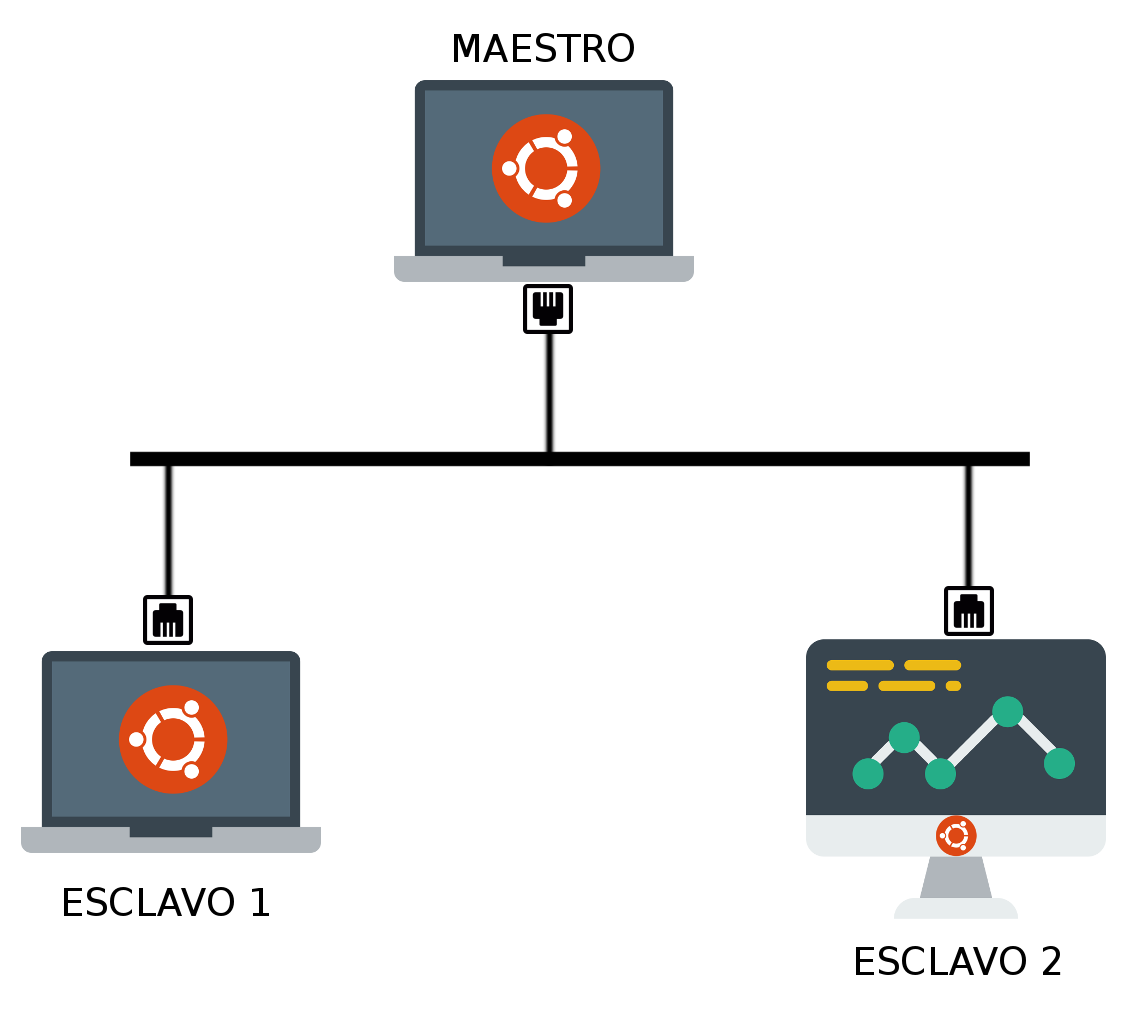
\includegraphics[scale=0.3]{graphics/clusterDomestico}
\end{figure}

Uno de los aspectos claves y diferenciadores con respecto al clúster universitario, es que en este no se cuenta con un \gls{NFS} por lo que para que todos los nodos del sistema cuenten con los datos se decide establecer un mecanismo de replicación de estos.

\textit{Apache hadoop} es la tecnología utilizada para montar este mecanismo de replicación mediante el uso de su sistema distribuido de ficheros (\gls{HDFS}) que resulta óptimo para esta configuración. Este mecanismo nos permitirá tener los datos en cada nodo del clúster y, así, lo único que circulará por la red serán las tareas que el maestro asigne a los esclavos y los resultados que estos obtengan tras su procesamiento. 

Esto evitará el tráfico que generaría transmitir los datos a procesar con la tarea asignada a los nodos esclavos, mejorando el rendimiento de la arquitectura.

\begin{figure}[htp!]
\centering
\caption{Esquema del sistema de replicación \gls{HDFS}}
\label{fig:hdfs}
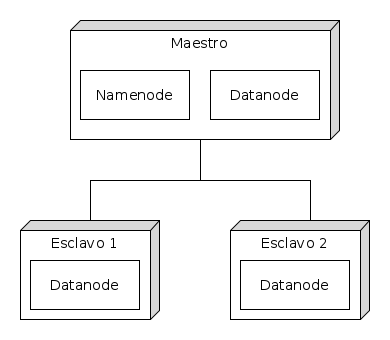
\includegraphics[scale=0.6]{diagramas/hadoop}
\end{figure}

Como se aprecia en la figura \ref{fig:hdfs} que muestra el esquema del sistema de replicación, para su funcionamiento, en cada nodo se necesita un proceso \textit{datanode} ejecutándose, que será el que se encargue de el almacenamiento de los datos en la máquina. Además, para controlar el estado de los \textit{datanodes} se necesita un proceso \textit{namenode}, que se ejecutará en el nodo maestro.

Debido a la buena interoperatividad de \textit{Apache Spark} con este sistema de replicación de datos, la implementación de este no implicará mayores cambios que la indicación de las rutas de los archivos a la que este sistema le asigne a los archivos manteniendo así la estructura de las unidades de procesamiento de los datos y las consultas.

Este diseño, tiene sus ventajas y desventajas con respecto a las demás configuraciones, pseudo-distribuida y multinodo universitario. En cuanto a las ventajas, la capacidad de procesamiento será mayor que la de el modo pseudo-distribuido al contar con un mayor número de núcleos y \gls{RAM}, aunque será menor que con respecto a la del clúster universitario al contar con menos nodos.

Otra de sus ventajas es la sencillez y el bajo coste que supone montar el sistema de replicación, en comparación con el \gls{NFS} del clúster universitario. Aunque tiene la desventaja del desaprovechamiento de espacio de disco en los nodos, donde cada uno tiene una copia de los datos aunque no los utilicen totalmente. Además, otra desventaja se produce al realizar el proceso de replicación, que debido a las limitaciones de la red, se realiza de forma lenta, necesitando un largo periodo de tiempo.

Finalmente, se puede comentar como desventaja que el nivel de configuraciones a realizar para montar este sistema es mayor que cualquiera de los otros que se implementarán debido a que, a parte de configurar \textit{Apache Spark}, habrá que configurar \textit{Apache Hadoop}.

\subsubsection{Clúster universitario \label{disUni}}
Como se ha indicado anteriormente, este clúster es el que representa un sistema \textit{big data} más realista, ya que, sus nodos tienen todos las mismas características y se dispone de un sistema de archivos en red que hace que el acceso a los datos sea más sencillo y eficiente. Además, la conexión entre los nodos se realiza a través de fibra óptica, obteniendo una velocidad superior al cable de red utilizado en el clúster doméstico.

Debido a la existencia de este sistema \gls{NFS} todos los nodos tienen acceso a los mismos datos que el nodo maestro, con la misma ruta de acceso, cosa que simplifica en gran manera la gestión de archivos. Además este sistema hace que no sea necesario un sistema de replicación, por lo que el proceso de  configuración del sistema es poco más complicado que el de la configuración pseudo-distribuida, diferenciándose únicamente en el procedimiento para conectar los nodos que formarán parte del clúster.

\begin{figure}[ht]
\centering
\caption{Arquitectura del clúster universitario}
\label{fig:clusterUni}
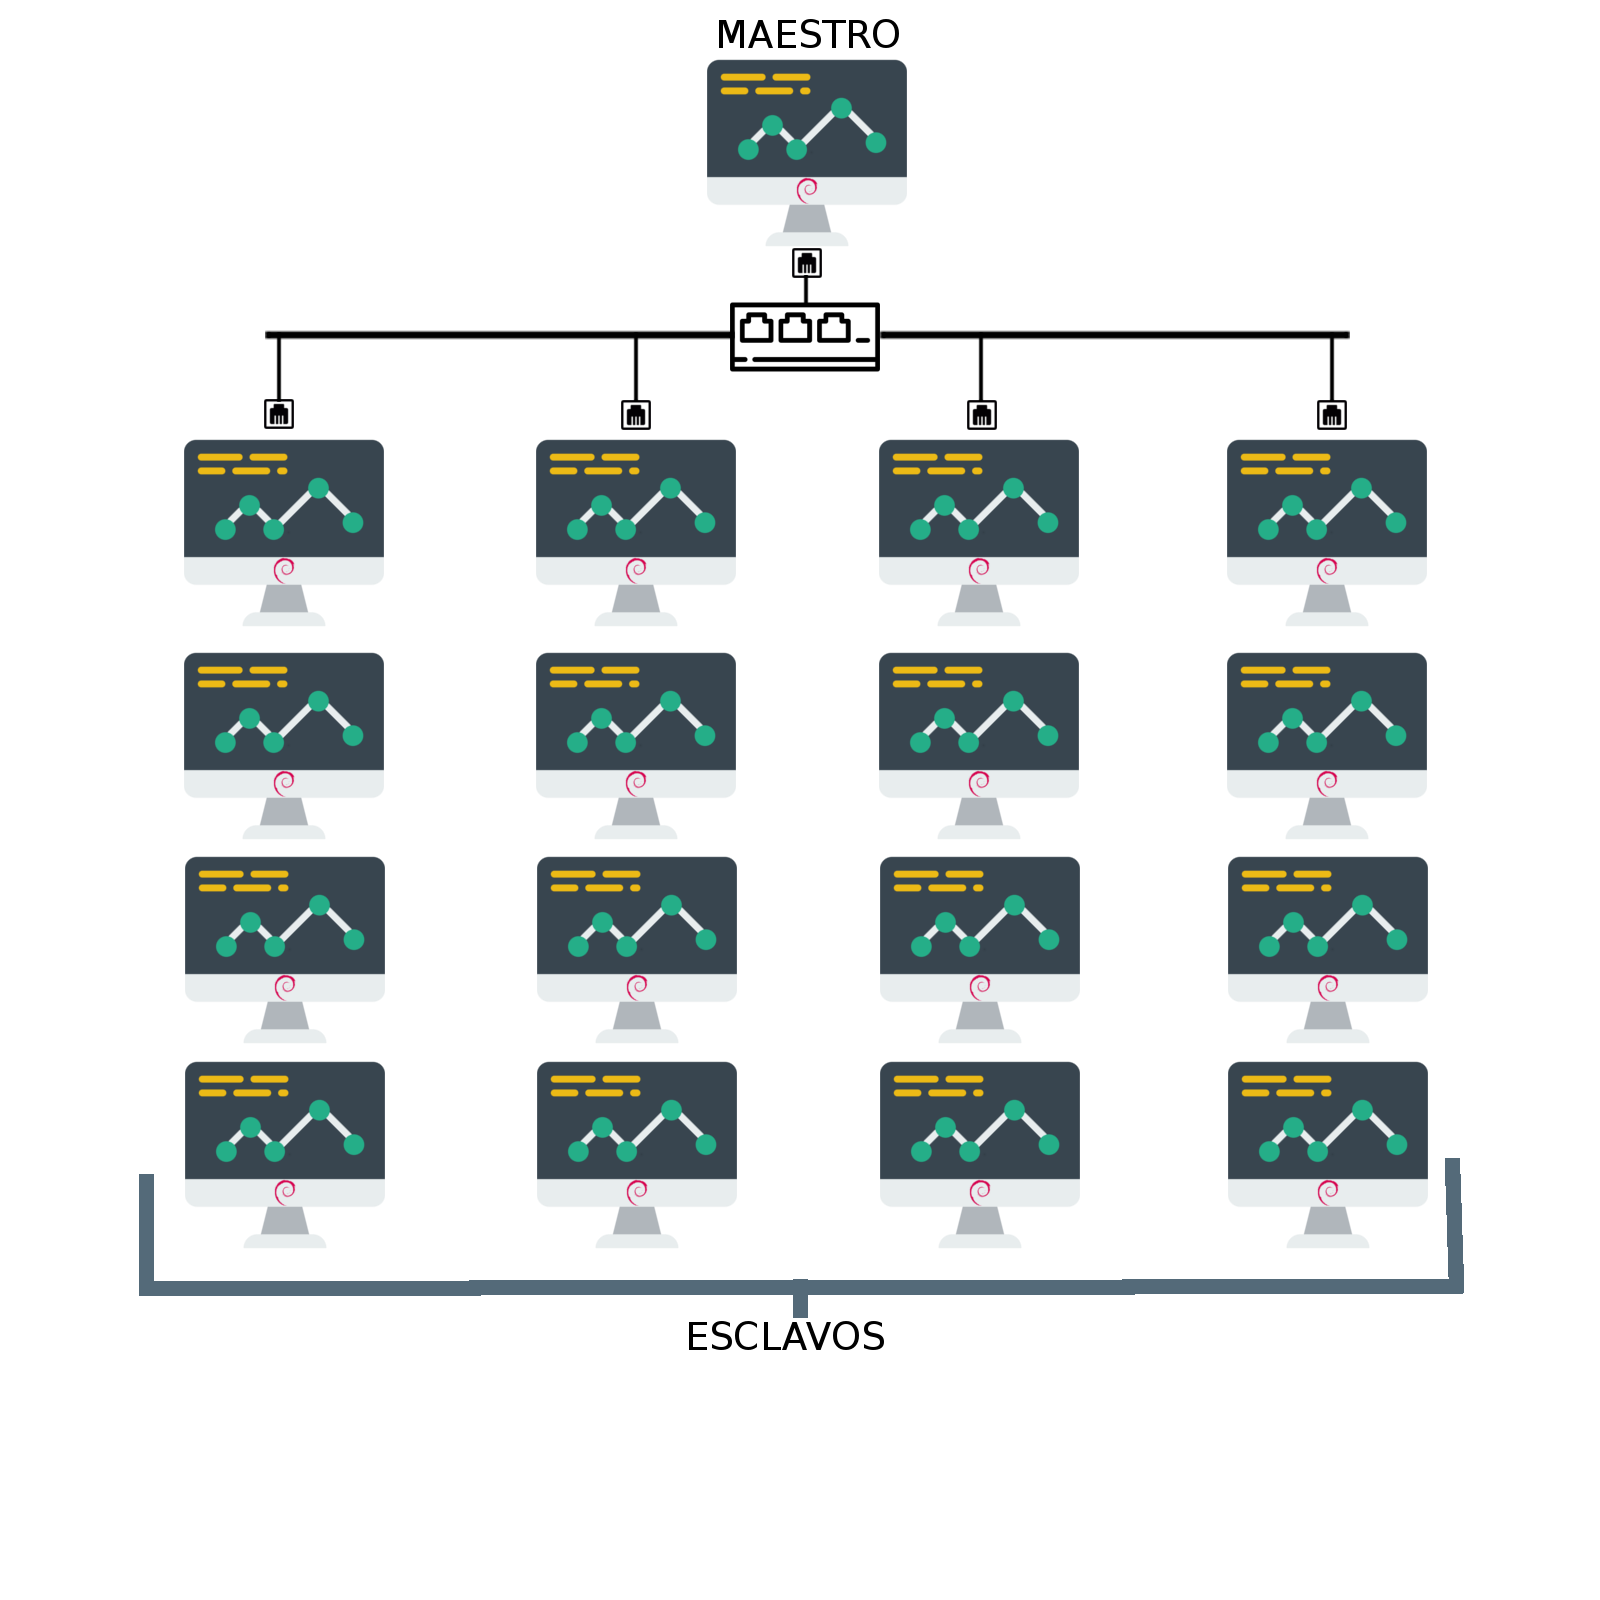
\includegraphics[scale=0.25]{graphics/clusterUni}
\end{figure}

En la figura \ref{fig:clusterUni} se puede apreciar la arquitectura de este clúster, este contará con un nodo que hará de maestro y que contendrá el objeto \textit{SparkContext} que será el encargado de distribuir las tareas entre todos los nodos y de recibir los resultados de estos y juntarlos para obtener los finales. El resto de nodos, que variarán en número para las diferentes pruebas, harán de esclavos. 

Este diseño, como todos los demás, tiene sus ventajas y desventajas. La principal ventaja es la capacidad de procesamiento que puede alcanzar, al contar con un alto número de nodos el número de \gls{CPU}s y gran cantidad de memoria \gls{RAM}, la capacidad de cálculo de esta configuración es elevada. Además, el sistema \gls{NFS} con conexiones de fibra óptica, hace que la velocidad de conexión sea elevada, permitiendo aprovechar la potencia de la arquitectura.

Por otro lado, este mismo sistema de ficheros hace que la configuración del sistema sea sencilla, ya que, no es necesario montar un mecanismo de replicación. Sin embargo, este también produce desventajas en el sistema, por un lado, tenemos una limitación en la cuota de disco a utilizar por el usuario, limitada a 30GB. Por otro lado, el coste de mantener este sistema es el más alto, debido al gran número de máquinas utilizadas para montarlo, así como para mantener el sistema de ficheros en red.

\section{Descripción de las unidades funcionales y sus componentes}
El sistema \textit{big data} estará compuesto por diferentes módulos que se relacionarán entre sí para el correcto funcionamiento del mismo, es decir, para que el flujo de las actividades y procesos a ejecutar sea continuo.

Como se ha comentado anteriormente, la implementación del sistema se realizará sobre dos entornos diferentes, uno doméstico, donde se contara con el sistema de replicación \gls{HDFS} y, otro universitario, donde se cuenta con un sistema \gls{NFS}. Esto hará que se presenten dos diseños para el almacenamiento de los datos, que aunque en su estructuración sean muy similares, tengan sus diferencias.

Por ello, como se indicó en el apartado \ref{unitFunc}, el sistema contará con tres unidades funcionales, dos de las cuales serán iguales para todas las configuraciones del sistema, la encargada del tratamiento de los datos y la obtención de resultados, y, una, la encargada de la carga y almacenamiento de los datos, que dependerá del sistema de ficheros usado.

En este apartado, por tanto, se describirá el diseño de las diferentes unidades funcionales del sistema, analizando los componentes que las forman y, tras ello, se tratarán las interacciones entre ellas y el usuario.

\subsection{Carga y almacenamiento de datos \label{diseñoFich}}
Esta unidad funcional será la única de la arquitectura que varíe dependiendo de la configuración que se utilice. Aunque la abstracción general será igual para los dos diseños, es decir, la estructura del sistema de ficheros será la misma, el diseño global no será el mismo por la diferencia en las características y funcionamiento de estos sistemas. 

Por tanto, diferenciaremos dos diseños, el primero que utilizará las herramientas ya disponibles en el sistema que será utilizado por el modo pseudo-distribuido, en ambos entornos, y por el modo distribuido en el entorno universitario, que al tratarse de un sistema \gls{NFS} funciona de la misma forma que el anterior. El segundo diseño será utilizado por el modo distribuido del clúster doméstico, que necesita del sistema de replicación \gls{HDFS} para su funcionamiento y que cambia el proceso de carga de datos y la estructura de almacenamiento.

El objetivo de este bloque funcional es alojar los datos a los que recurrirá el sistema para realizar el resto de tareas, ya sea el tratamiento de los mismos o el análisis para obtener los resultados a las consultas. Por tanto, al diferenciarse dos tipos de datos, unos, cargados por el usuario y sin procesar y, otros, ya tratados por el sistema, el diseño deberá contemplar una separación entre ellos. Además, el usuario también tendrá que ser capaz de acceder a los ficheros de los resultados, que también serán almacenados en el sistema.

\begin{figure}[htp!]
\centering
\caption{Estructura general para el almacenado de datos}
\label{fig:estructAlmacen}
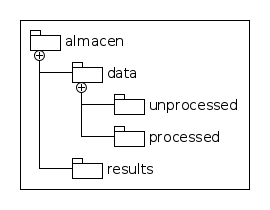
\includegraphics[scale=0.8]{diagramas/estrucAlmacen}
\end{figure}

Por tanto, la estructura del sistema de ficheros, independientemente de la implementación, tendrá una organización como se puede observar en la figura \ref{fig:estructAlmacen}, donde cada tipo de dato que maneje el sistema tendrá un apartado específico.

Por un lado, se diferenciará entre los datos con los que trabajará el sistema, es decir, las trazas de los taxis, que serán almacenadas en la carpeta ``data'' y, dentro de esta, se distinguirá también entre los ficheros cargados por el usuario, que irán destinados a la carpeta ``unprocessed'' y los tratados por el sistema, que se almacenarán en la carpeta ``processed'', a los que accederá el sistema para obtener los resultados de las consultas. Con respecto a esto resultados, serán almacenados en una carpeta diferenciada de los datos.

\subsubsection{Diseño para la configuración pseudo-distribuida y la distribuida universitaria \label{disNormal}}
Gracias al diseño de \textit{Apache Spark}, como se indicó en el apartado \ref{sparkEA}, este permite la lectura de ficheros directamente desde el disco, si tener que estar contenidos en ningún tipo de gestor de ficheros específico, del tipo \gls{HDFS}. Por tanto, aprovechando la sencillez que esto supone, este diseño cuenta con el sistema de ficheros propio del \gls{SO}, donde se establecerá la estructura mostrada en la figura \ref{fig:esquemagen}.

Por tanto, la carga de datos por el usuario en este sistema será muy sencillo, únicamente teniendo que copiar el fichero deseado en la carpeta correspondiente, en este caso, al cargar ficheros sin tratar, en la ruta ``/almacen/data/unprocessed''. Con respecto a la obtención de los resultado, solo tendría que navegar a la carpeta que los contiene.

\subsubsection{Diseño para la configuración distribuida doméstica \label{disHDFS}}
En este caso, al necesitar de un sistema de replicación para el funcionamiento correcto de esta configuración, el diseño será diferente para ajustarse a los requerimientos de este mecanismo, que en este caso es el sistema de ficheros que proporciona \textit{Apache Hadoop},  como se ha indicado en el apartado \ref{disDomestico}.

La diferencia con el otro diseño, por un lado, será la estructura en disco que presentará el sistema en los diferentes nodos, debido a los requerimientos del \gls{HDFS} en cuanto a esta y, por otro, la forma de cargar y acceder a los datos por parte del usuario y de los demás componentes del sistema.

Con respecto a la estructura de este diseño, para el correcto funcionamiento del sistema de replicación, este necesita que en cada nodo del clúster exista una carpeta llamada ``datanode'' que será donde se repliquen los datos, además, necesita otra carpeta para archivos temporales. El nodo maestro, para controlar el proceso de replicación, necesita una carpeta llamada ``namenode''.

Por tanto, para mantener una estructura de carpetas similar a la planificada inicialmente, se decidió crear dentro del \gls{HDFS} las carpetas ``unprocessed'' y ``processed'', donde guardar las trazas de los taxis, que son los datos que necesitarán los nodos esclavos. Con respecto a la carpeta donde guardar los resultados, esta solamente existirá en la máquina maestra, que es a la que la que manipula el usuario, considerando el replicar estos ficheros en los nodos esclavos poco útil y eficiente.

\begin{figure}[htp!]
\centering
\caption{Esquema de la estructura del almacén de datos en el clúster doméstico}
\label{fig:esquemahdfs}
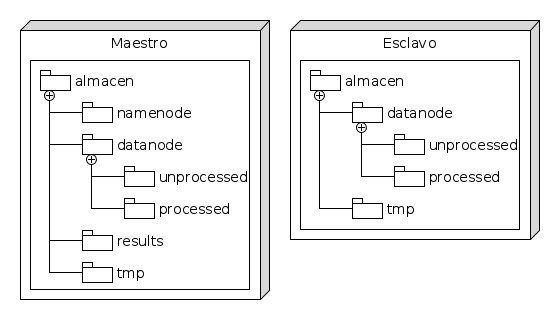
\includegraphics[scale=0.7]{diagramas/esquemahdfs}
\end{figure}

Tras estas decisiones, el esquema resultante es el de la figura \ref{fig:esquemahdfs}. En este podemos apreciar que los nodos contienen las carpetas necesarias para el correcto funcionamiento del \gls{HDFS}. Teniendo el maestro, a parte de la necesaria para controlar el proceso de replicación, la carpeta donde se almacenarán los resultados.

En cuanto a la carga y acceso de los datos de las trazas, veremos en el apartado \ref{sec:implementación}, como las rutas no serán convencionales, como en el diseño del apartado \ref{disNormal}, y se necesitarán unos comandos específicos de \textit{Apache Hadoop} para su manipulación. Con respecto a los resultados, al ser almacenados únicamente en el maestro, si utilizarán el sistema de ficheros del sistema y su comportamiento si que será igual que en el otro diseño.

\subsection{Procesamiento de datos}
Esta unidad funcional será la que se encargue de limpiar las trazas inválidas y transformar los datos de los ficheros que carga el usuario en el sistema. Esta transformación de los datos se da debido a los diferentes requisitos de la competición y se tratará detalladamente durante la implementación del sistema, en el apartado \ref{anaProcData}.

Estará compuesta por una sola clase, escrita en Python, que obtendrá el fichero sin procesar cargado por el usuario en primer lugar y que, tras realizar las transformaciones necesarias lo guardará en el espacio de los archivos procesados, para que pueda ser utilizado por el resto del sistema.

\subsection{Obtención de resultados \label{disConsultas}}
Este bloque de funcionamiento será el encargado de analizar los datos ya procesados y obtener los resultados a la consulta realizada. Estas consultas, que son las establecidas en la competición \cite{grandChallenge}, son las siguientes:

\begin{itemize}
\item \textbf{Rutas más frecuentes:} El objetivo es obtener las diez rutas más frecuentes dentro de la ventana de tiempo establecida entre una fecha y hora dada y la media hora anterior.

\item \textbf{Zonas que más beneficios aportarían al taxista:} El objetivo es obtener las diez zonas de Nueva York donde un taxista obtendría el mayor beneficio empezando un viaje desde allí. Esta consulta también tomaría como entrada una fecha y hora y establecería como ventana de tiempo los 15 minutos anteriores a esta.
\end{itemize}

Estas serían las dos consultas originales de la competición, pero, además, como decisión propia para llevar más al límite a la arquitectura se hicieron modificaciones a estas consultas para tener en cuenta la estacionalidad en los resultados, desarrollando otras dos consultas:

\begin{itemize}
\item \textbf{Rutas más frecuentes teniendo en cuenta la estacionalidad:} El objetivo sigue siendo conseguir las diez rutas más frecuentes pero teniendo en cuenta los viajes de todo el año, dando más importancia a los más cercanos al mes y al día determinado en la consulta. Es decir, esta contará como entrada un mes, un día de la semana y la hora deseada y la consulta obtendrá las rutas más frecuentes teniendo los viajes de todo el año ese día de la semana y a esa hora.

\item \textbf{Zonas que más beneficios aportarían al taxista:} El objetivo es obtener las diez zonas de Nueva York donde un taxista obtendría el mayor beneficio empezando un viaje desde allí. Esta consulta, al igual que la anterior, también tiene en cuenta todos los viajes del año, aunque dando más valor a las fechas cercanas a los argumentos introducidos.
\end{itemize}

Estas consultas, al tener en consideración una franja de tiempo más amplia necesitan más procesamiento para ser calculadas. Además, para aumentar este requerimiento, se ha diseñado para establecer factores de relevancia a los viajes según su cercanía a la fecha introducida.

Por tanto, el sistema contará con la posibilidad de realizar cuatro consultas cuya implementación serán detalladas en el apartado \ref{impConsultas}. El esquema de esta unidad funcional queda representado en la figura \ref{fig:consultas}. 

\begin{figure}[htp!]
\centering
\caption{Esquema de la unidad funcional encargada de realizar las consultas y devolver los resultados}
\label{fig:consultas}
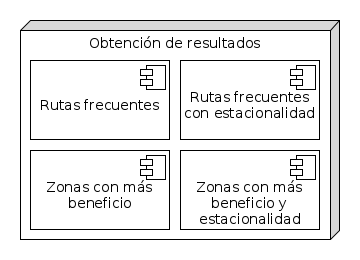
\includegraphics[scale=0.7]{diagramas/obtResultados}
\end{figure}

Con respecto a los resultados de las consultas, estos se guardarán en un archivo con el nombre de la consulta realizada y serán almacenados en la carpeta del almacén de datos destinada para ello, la carpeta ``results''.

\section{Interacciones del sistema}
\begin{figure}[htp!]
\centering
\caption{Componentes e interacciones del sistema \textit{big data}}
\label{fig:interacciones}
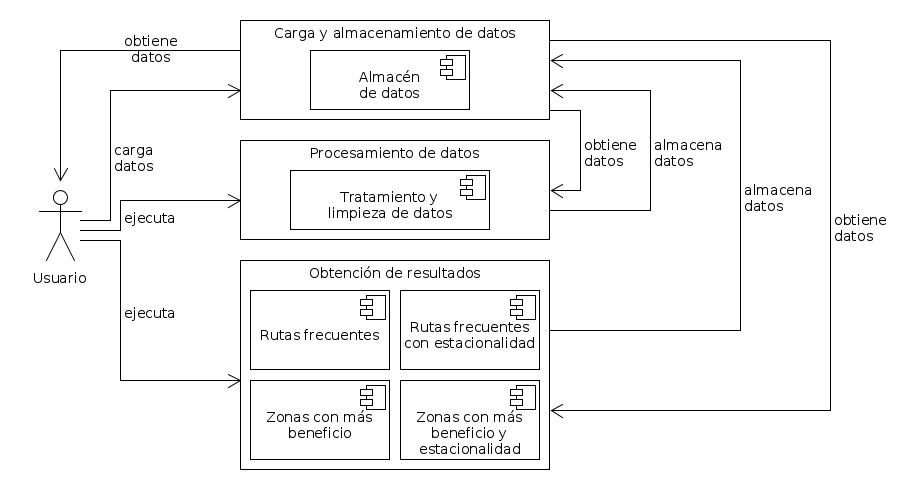
\includegraphics[scale=0.52]{diagramas/interacciones}
\end{figure}

Una vez descritas las diferentes unidades funcionales del sistema y los componentes que las componen, en la figura \ref{fig:interacciones} podemos encontrar un esquema general de las interacciones que se dan entre el usuario y el sistema y, dentro del mismo, entre los diferentes componentes.

En este apartado, además, vamos a detallar las interacciones que se producen al realizar las tareas que la arquitectura puede realizar. Estas tareas son las siguientes: carga de datos en el sistema por parte del usuario, tratamiento y limpieza de los datos, ejecución de las consultas, obtención de los resultados.

\subsection{Carga de datos}
\begin{figure}[htp!]
\centering
\caption{Diagrama de interacción para realizar la carga de los datos}
\label{fig:cargaDatos}
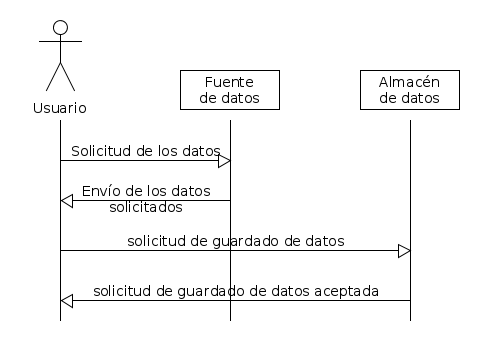
\includegraphics[scale=0.7]{diagramas/cargaDatos}
\end{figure}

Comprende la parte en la que el usuario del sistema carga la traza de taxis, obtenida de la página de la competición. En ella el usuario descarga la traza y la introduce en el sistema mediante su copia en el almacén de datos. Figura \ref{fig:cargaDatos}.

\subsection{Tratamiento y limpieza}

\begin{figure}[htp!]
\centering
\caption{Diagrama de interacción para realizar el tratamiento y la limpieza de los datos}
\label{fig:procesamientoDatos}
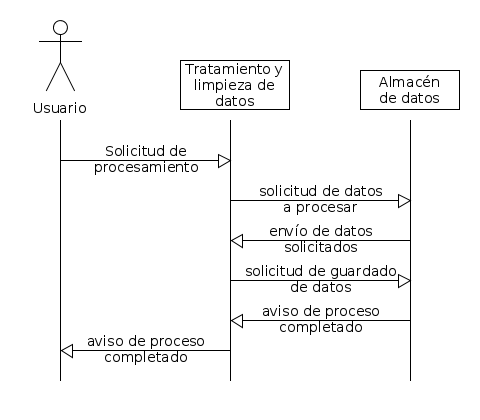
\includegraphics[scale=0.7]{diagramas/procesamientoDatos}
\end{figure}

Este proceso comprende la limpieza y transformación de los datos, procesos necesarios para poder realizar la consulta sobre la traza de datos cargado anteriormente. En este, el usuario realiza una petición de procesamiento al componente con nombre del archivo sin procesar a tratar, que, a su vez, realiza la petición del archivo al almacén de datos. Tras obtener el fichero, este lo trata y realiza el guardado del fichero procesado en el disco, avisando al usuario al finalizar el proceso. Figura \ref{fig:procesamientoDatos}.

\subsection{Ejecución de las consultas}
\begin{figure}[htp!]
\centering
\caption{Diagrama de interacción para realizar las consultas sobre los datos}
\label{fig:consulta}
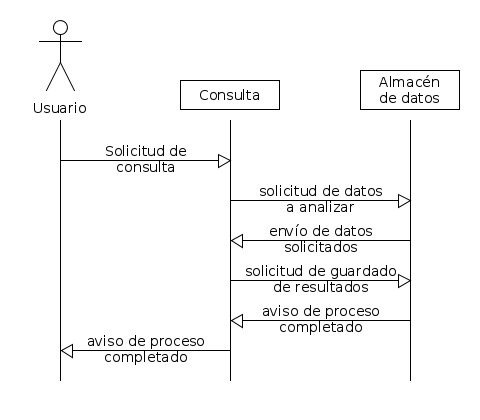
\includegraphics[scale=0.7]{diagramas/consulta}
\end{figure}

Comprende la ejecución de la consulta deseada por el usuario sobre el fichero procesado indicado. Para ello, el usuario realiza una petición al sistema con la consulta que quiere ejecutar y el archivo sobre el que realizarla. Además de indicar los datos requeridos por la consulta. Una vez realizada la petición, el componente de consultas realiza una solicitud al almacén para obtener los datos sobre los que realizará el análisis. Tras realizar el análisis y obtener los resultados, se realiza la petición al almacén para guardarlos y se avisa al usuario de que se ha completado la tarea. Figura \ref{fig:consulta}.

\subsection{Obtención de resultados}
\begin{figure}[htp!]
\centering
\caption{Diagrama de interacción para obterner los resultados de la consulta}
\label{fig:pedirRes}
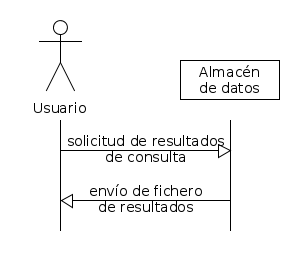
\includegraphics[scale=0.7]{diagramas/pedirRes}
\end{figure}

Este proceso comprende la parte donde el usuario obtiene el fichero de resultados creado tras una consulta ejecutada anteriormente. En este, el usuario realiza una petición al almacén indicando la consulta realizada y este devolverá el fichero con los resultados.
